\documentclass[12pt, oneside]{article} 
\usepackage[a4paper]{geometry}              
\usepackage{graphicx}
\usepackage{amsmath}
\usepackage{amssymb}
\usepackage[table]{xcolor}

%SetFonts
\usepackage[T1]{fontenc}
\usepackage[bitstream-charter]{mathdesign}
%SetFonts

%define example environment 
\newcounter{examplecounter}
\newenvironment{example}%
{%
\small\begin{quote}%
\refstepcounter{examplecounter}%
\textbf{Example \arabic{examplecounter}}%
\quad%
}%
{%\schluss%
\end{quote}%
}

%define remark environment 
\newcounter{remarkcounter}
\newenvironment{remark}%
{%
\small\begin{quote}%
\refstepcounter{remarkcounter}%
\textbf{Remark \arabic{remarkcounter}}%
\quad%
}%
{%\schluss%
\end{quote}%
}

%define remark environment 
\newcounter{questioncounter}
\newenvironment{question}%
{%
\small\begin{quote}%
\refstepcounter{questioncounter}%
\textbf{Question \arabic{questioncounter}}%
\quad%
}%
{%\schluss%
\end{quote}%
}


%define important environment
\newenvironment{important}{\begin{quote}%
\textbf{Important:}%
\quad
}{%
\end{quote}%
}

\newcommand{\qed}{\nobreak \ifvmode \relax \else
      \ifdim\lastskip<1.5em \hskip-\lastskip
      \hskip1.5em plus0em minus0.5em \fi \nobreak
      \vrule height0.5em width0.5em depth0.25em\fi}

\newtheorem{theorem}{Theorem}[section]
\newtheorem{corollary}{Corollary}[section]
\newtheorem{lemma}[theorem]{Lemma}
\newtheorem{proposition}[theorem]{Proposition}
\newtheorem{definition}{Definition}
\newenvironment{proof}[1][Proof]{\begin{trivlist}
\item[\hskip \labelsep {\bfseries #1}]}{\end{trivlist}}

\newcommand{\R}{\mathbb{R}}
\newcommand{\C}{\mathbb{C}}
\newcommand{\E}{\mathbb{E}}
\newcommand{\F}{\mathbb{F}}
\newcommand{\range}{\text{\normalfont range}}
\newcommand{\rank}{\text{\normalfont rank}}
\newcommand{\fol}{\mathcal{F}}
\newcommand{\one}{\mathbb{1}}
\newcommand{\hest}{\textsc{Hesten}}
\newcommand{\texp}{T_{\rm exp}}
\newcommand{\detp}{{\det}_+}

\usepackage{lettrine}

\begin{document}
\noindent{\Huge \textbf\textsf{{Comment on Taleb's Bitcoin Paper}}}

\noindent \textit{by Olaf Dreyer}

\vspace{.5cm}

\section{Setup}
We use the standard setup to describe a foreign exchange market. We thus have two interest rates and one exchange rate. Let 
\begin{equation}
	P_E(t,T)
\end{equation}
be the discount factor for the base currency and let 
\begin{equation}
	P_B(t,T)
\end{equation}
be the discount factor for the foreign currency. In our example the foreign currency will be bitcoin itself. 

\begin{remark}
	The introduction of a discount factor for bitcoins might seem unusual. This is standard praxis in the description of different assets classes including proper currencies, inflation, equities, and commodities. See \cite{brigo}, \cite{clark1}, and \cite{clark2} for more details (in \cite{brigo} this is called the 'The Foreign-Currency Analogy').
\end{remark}

The exchange rate at time $t$ between the base currency and bitcoins is denoted by
\begin{equation}
	X(t).
\end{equation}
The rate $X(t)$ give the value of one bitcoin $B$ in the base currency $E$. 

A complete description of the bitcoin market would now consists of models for the two discount factors $P_E$ and $P_B$ together with a model for the exchange rate $X$. 

\begin{example}
	The simplest model of this kind would be a model where the interest rates are non-stochastic and the exchange rate is modeled by a simple Black-Scholes model:
	\begin{equation}
		\frac{dX}{X} = \mu dt + \sigma dW
	\end{equation}
	The price of a bitcoin option would then be given by a Garman-Kohlhagen type formula:
	\begin{equation}
	V(t) = P_E(t,T) \bigg( F(t,T) N_{(0,1)} \left[ d_1 \right] - K N_{(0,1)} \left[ d_2 \right] \bigg),
\end{equation}
with
\begin{equation}
	d_{1/2} = \frac{\ln\left(\frac{F(t,T)}{K}\right) \pm \frac{1}{2}\sigma^2 T}{\sigma\sqrt{T}},
\end{equation}
where $F(t,T)$ is the forward:
\begin{equation}
	F(t,T) = X(t) \frac{P_B(t,T)}{P_E(t,T)}
\end{equation}
We will see more of the forward in a bit.
\end{example} 

We will not specify a particular model here but rely on arguments that are model-independent. 

\section{The forward}
Let us calculate the value of the payment of one bitcoin at time $T$. This value is given by
\begin{equation}
	V(t) = E\left[\frac{X(T)}{N(T)}\right],
\end{equation}
where $N(T)$ is the standard money market account for the base currency $E$. We now perform two changes of numeraire. First we transform to the forward measure with the numeraire
\begin{equation}
	M(t) = P(t,T).
\end{equation}
This gives
\begin{equation}\label{eqn.forw1}
	V(t) = P_E(t,T) E^T[ X(T) ],
\end{equation}
where $E^T[\cdot]$ is the expectation with respect to the forward measure. Transforming instead to the foreign forward measure using the numeraire 
\begin{equation}
	M(t) = X(t) P_B(t,T)
\end{equation}
gives
\begin{align}
	V(t) & = X(t) P_B(t,T) \\
	& = P_E(t,T) X(t,T)\label{eqn.forw2},
\end{align}
where we have introduced the forward exchange rate
\begin{equation}\label{eqn.defforward}
	X(t,T) = X(t) \frac{P_B(t,T)}{P_E(t,T)}.
\end{equation}
Comparing equation (\ref{eqn.forw1}) with equation (\ref{eqn.forw2}) gives
\begin{equation}\label{eqn.forwexp}
	X(t,T) = E^T[ X(T) ].
\end{equation}
The forward exchange rate is thus given by the expectation value of $X(T)$ in the forward measure.

\section{Taleb's argument}
Using the language of the previous sections we can now reformulate Taleb's argument as follows:

Usually $X(t)$ is used to calculate the forward $X(t,T)$. Taleb argues in the other direction. He uses the knowledge of the forward $X(t,T)$ to calculate $X(t)$. It follows from equations (\ref{eqn.defforward}) and (\ref{eqn.forwexp}) that
\begin{align}
	X(t) & = \frac{P_E(t,T)}{P_B(t,T)} X(t,T) \\
	& = \frac{P_E(t,T)}{P_B(t,T)} E^T[ X(T) ].\label{eqn.xoft}
\end{align}
Taleb argues that for $T$ large enough all paths will have seen the exchange rate $X(T)$ dip below the absorbing boundary (see appendix \ref{app.boundary}) and thus vanish, i.e.
\begin{equation}
	\lim_{T\rightarrow \infty} E^T[ X(T) ] = 0.
\end{equation}
It then follows from equation (\ref{eqn.xoft}) that $X(t)$ (i.e. the value of bitcoin today) also vanishes.



\appendix


\section{The absorbing boundary}\label{app.boundary}
\subsection{The reflection principle}\label{sec:brownianmotion}
Let $W(t)$ be a Brownian motion. Let us denote by $\tau_A$ the first time a path of the Brownian motion had the value $A$. Let us introduce the set of paths $W(t)$ for which $\tau_A\le T$ but which have a value $W(T)$ that is larger than $w>A$:
\begin{equation}
	C_A(T,w) = \left\{ W(t) \vert \tau_A\le T \text{ and } W(T)>w\right\}
\end{equation}
An example of an element of $C_A(T,w)$ is the red path shown in figure \ref{fig:reflection}. Let us change this path by mirroring the part of the path after $\tau_A$ on the line given by $A$. The new path thus goes up when the original path goes down and down when the original path goes up. In figure \ref{fig:reflection} this is the blue path. This paths now ends up at a value that is smaller than
\begin{equation}
	A - (w-A) = 2 A - w.
\end{equation}
Let us thus introduce the set of paths that are smaller than a given value at time $T$:
\begin{equation}
	D(T,v) = \left\{ W(t) \vert W(T)<v\right\}
\end{equation}
Following the above argument we have shown that there is a one-to-one correspondence between $C_A(T,w)$ and $D(T,2A-w)$. For the standard Brownian motion that we are looking at it follows that the probabilities of these sets are equal:
\begin{equation}
	P( C_A(T,w) ) = P( D(T,2A-w) )
\end{equation}
This is called the \emph{reflection principle}.

\begin{center}
\begin{figure}[hbt]
  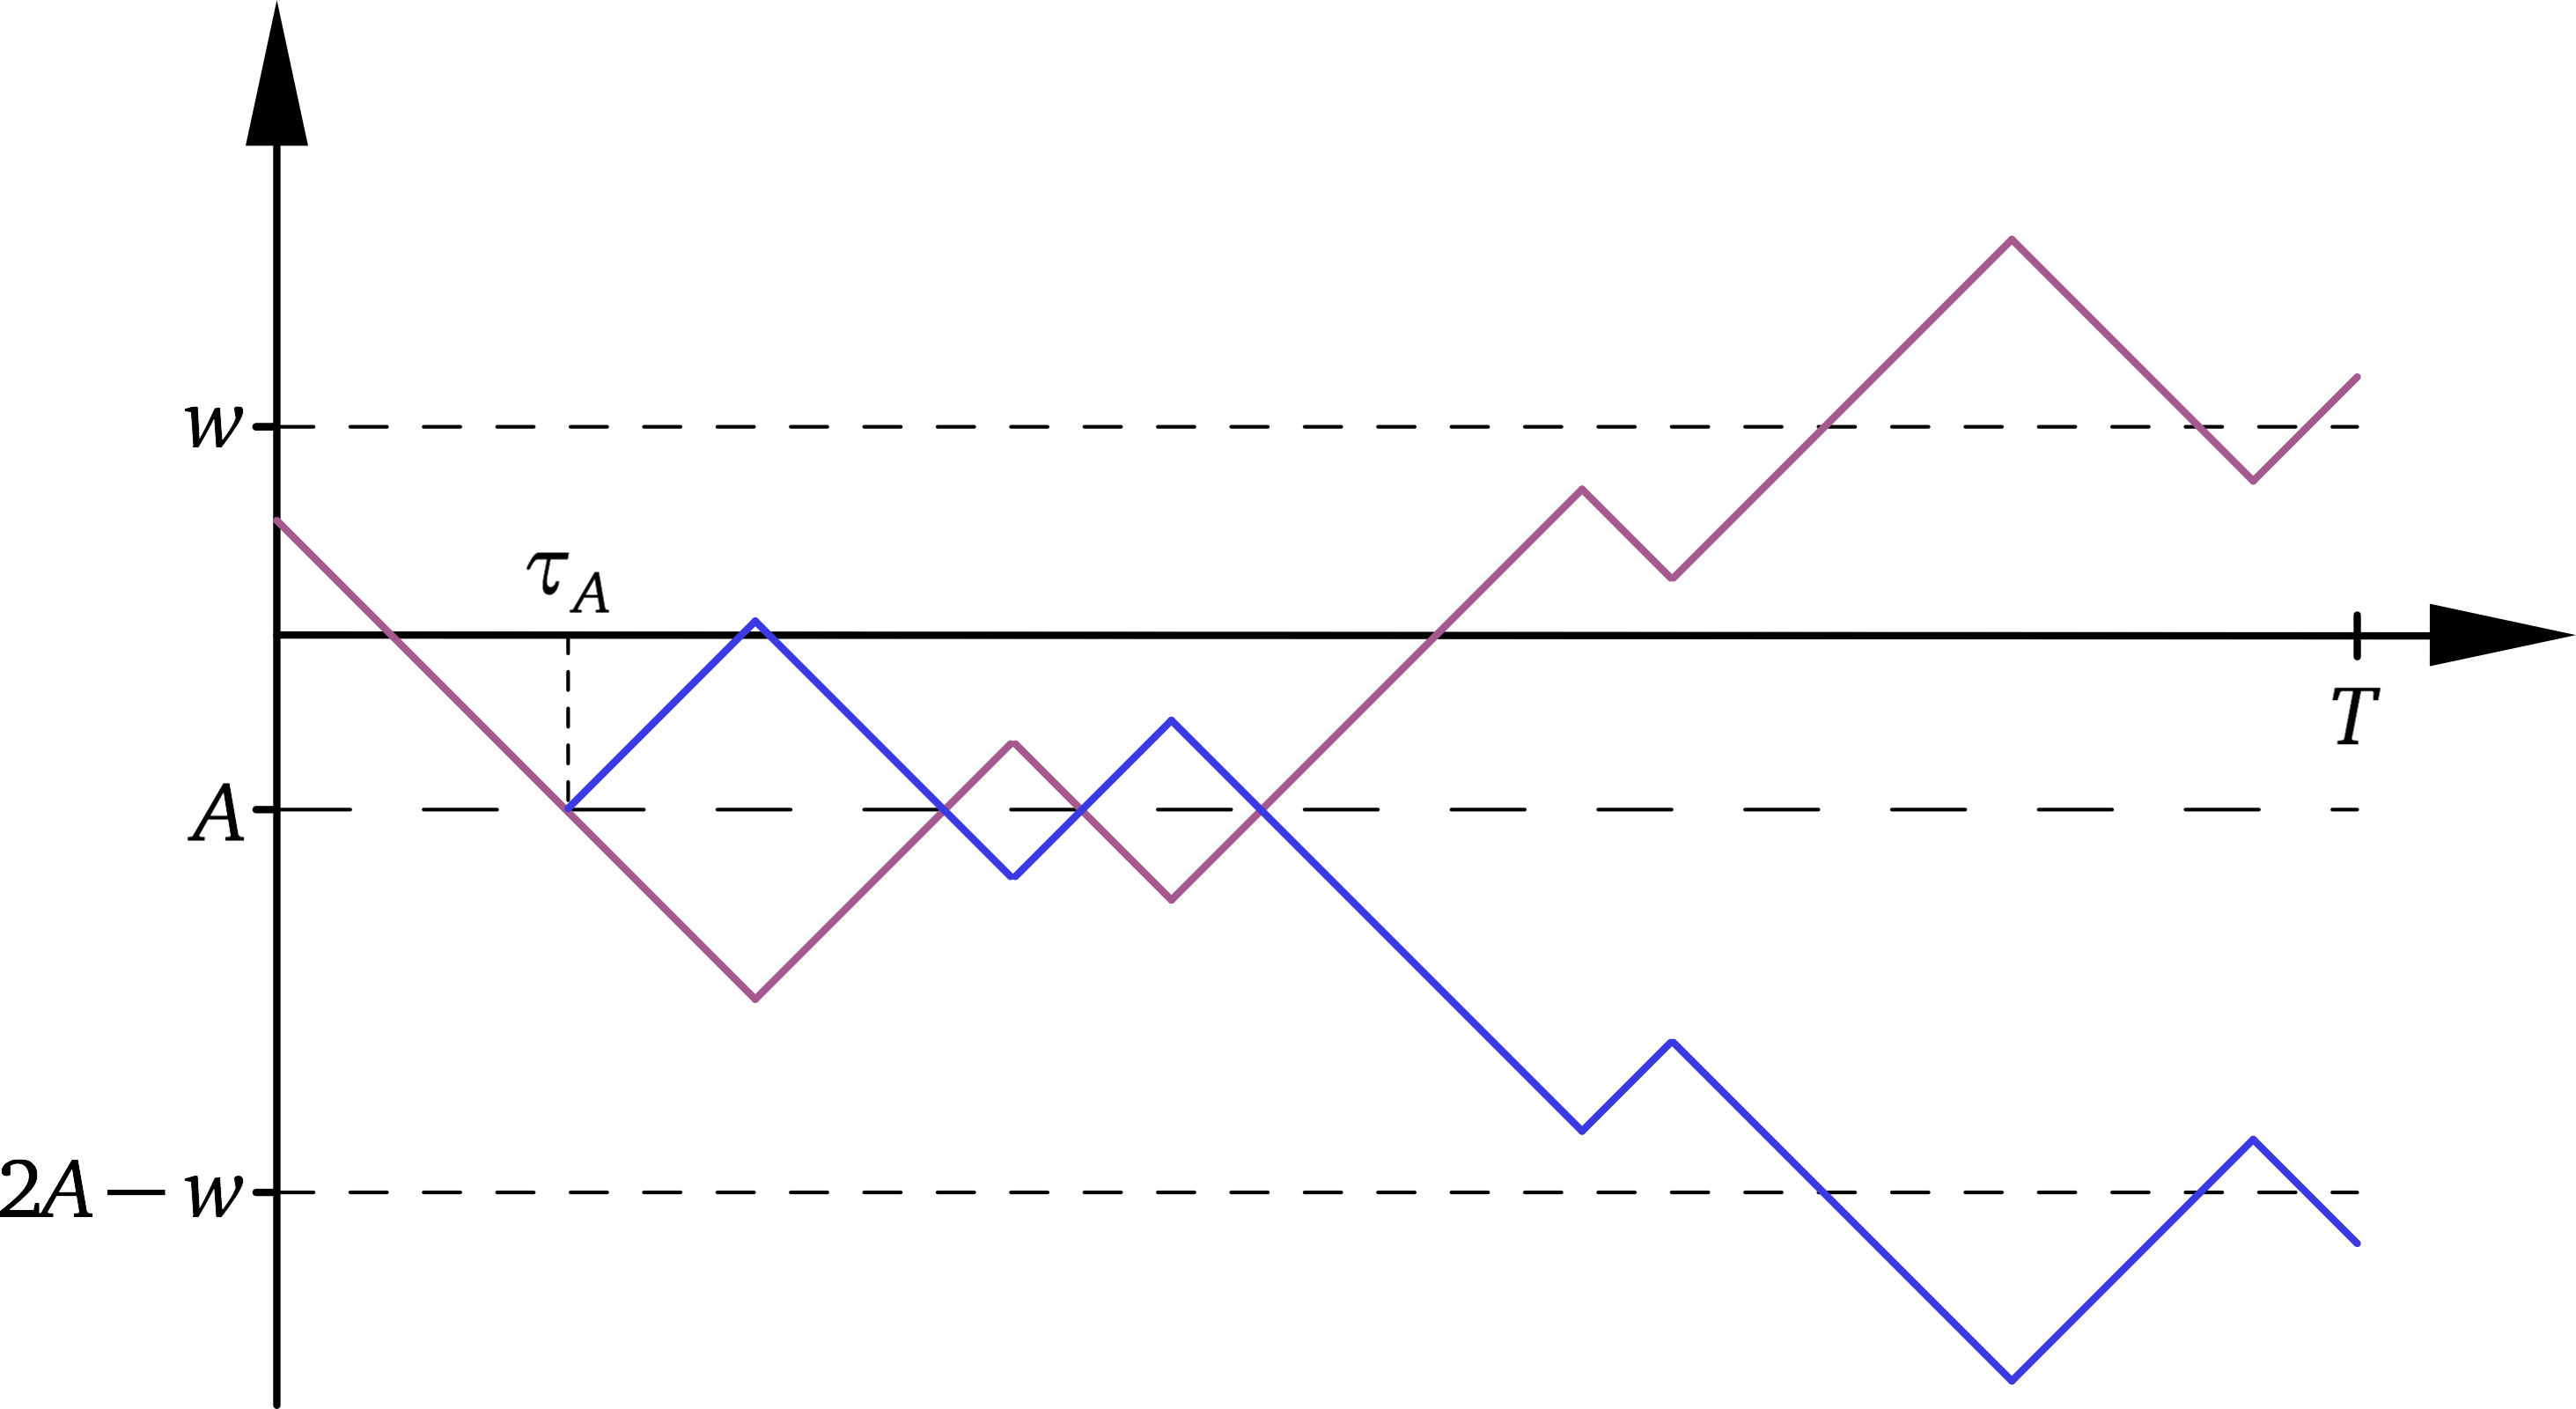
\includegraphics[width=12cm]{reflectionPrinciple.png}
  \caption{For every path that assumes the value $A$ at any time before $T$ (i.e. a path for which $\tau_A\le T$) but that has a value $W(T)> w$ there is a path for which $W(T)<2A-w$. In this figure the red path crosses $A$ at time $\tau_A$ but has a value larger than $w$ at time $T$. The blue path is obtained by reflecting the red path around the dashed line at $A$. It ends lower than $2A-w$.}\label{fig:reflection}
\end{figure}	
\end{center}

\subsection{The absorbing boundary}
We will use the reflection principle to deal with the absorbing  boundary. The Brownian motion that we were looking at in the last section is the exchange rate $X(t)$. We want to know how many paths of $X$ have been below a certain value $A$ at time $T$. A complication arises because we assume that the boundary is absorbing. If we just counted the paths that are below $A$ at time $T$ we would miss out on those paths that dipped below $A$ at a time $\tau<T$. The set of paths that should be counted as having zero exchange rate at time $T$ thus splits into two sets. There is the set of paths with $X(T)<A$ and then there is the set of paths $X(\tau)<A$ for some $\tau<T$ but with $X(T)>A$.

We can use the notation of the last section to denote these sets. The set of paths for which $X(T)>A$ is
\begin{equation}
	D(T,A).
\end{equation} 
The other set of paths is given by
\begin{equation}
	C_{A}(T,A).
\end{equation}
Let us make the connection to the last section explicit:
\begin{align}
	A &\simeq A \\
	w &\simeq A \\
	\tau_A &\simeq \tau
\end{align}
The reflection principle then says that these two sets have the same probability:
\begin{equation}
	P(C_{A}(T,A)) = P( D(T,A) )
\end{equation}
We need to count \emph{both} of these sets. The probability that the exchange rate vanishes is thus
\begin{equation}
	p_0 = 2 P( D(T,A) ).
\end{equation}
When the width $\sigma$ of the Brownian motion goes to infinity we have
\begin{equation}
	\lim_{T\rightarrow\infty} P( D(T,A) ) = \frac{1}{2},
\end{equation}
for any value of $A$. We thus have
\begin{equation}
	\lim_{T\rightarrow\infty} p_0 = 1.
\end{equation}


\begin{thebibliography}{WW}
	\bibitem{brigo} Damiano Brigo, \emph{Fabio Mercurio, Interest Rate Models -- Theory and Practice, With Smile, Inflation and Credit}, 2nd Edition, Springer, 2006.
	\bibitem{clark1} Iain J. Clark, \emph{Foreign exchange option pricing: a practitioner's guide}, Wiley, 2011.  
	\bibitem{clark2} Iain J. Clark, \emph{Commodity Option Pricing: a practitioner's guide}, Wiley, 2014.  
\end{thebibliography}

\end{document}